
\begin{frame}{Content}{}
\tableofcontents
\end{frame}

%-------------------------------------------------------
%-------------------------------------------------------
\section{Introduction}
%-------------------------------------------------------
%-------------------------------------------------------
%%%%%%%%%%%%%%%%%%%%%%%%%%%%%
%         SLIDE             %
%%%%%%%%%%%%%%%%%%%%%%%%%%%%%
\begin{frame}
  \frametitle{Particle physics: today and future}

  \begin{itemize}
  \item The Large Hadron Collider (LHC) is today's largest particle
    accelerator at CERN (European Organisation for Nuclear Research)
    \begin{itemize}
    \item Proton-proton collisions
    \item Center-of-mass energy: $\sqrt{s}=13\,\tev$
    \item Observation of the Higgs boson in 2012
    \end{itemize}

  \item Still open questions in particles physics remain unanswered:
    \begin{itemize}
    \item Full understanding of the Higgs boson
    \item The origin of matter-antimatter asymmetry
    \item Dark matter
    \item Many more questions ...
    \end{itemize}

  \item Several approaches of high-energy particle colliders to
    address the unanswered questions in the post-LHC era:
    \begin{itemize}
    \item proton-proton ($p~p$) colliders
      \\
      \textcolor{Red}{and/or}
      \\
    \item electron-positron ($e^+e^-$) colliders
    \end{itemize}
  \end{itemize}

\end{frame}

%%%%%%%%%%%%%%%%%%%%%%%%%%%%%
%         SLIDE             %
%%%%%%%%%%%%%%%%%%%%%%%%%%%%%
\begin{frame}
  \frametitle{Hadron vs. Lepton colliders $\Rightarrow$ Discovery to Precision}
  
  % \begin{block}{}
  %   \centering
  %   Discovery to Precision
  % \end{block}

  \begin{columns}[t]
    \column{0.5\textwidth}
    \centering
    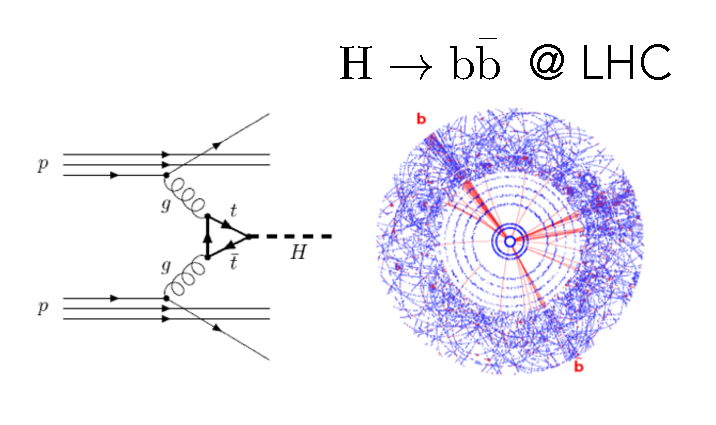
\includegraphics[width=0.6\textwidth]{figures/hadronColliders.pdf}

    \column{0.5\textwidth}
    \centering
    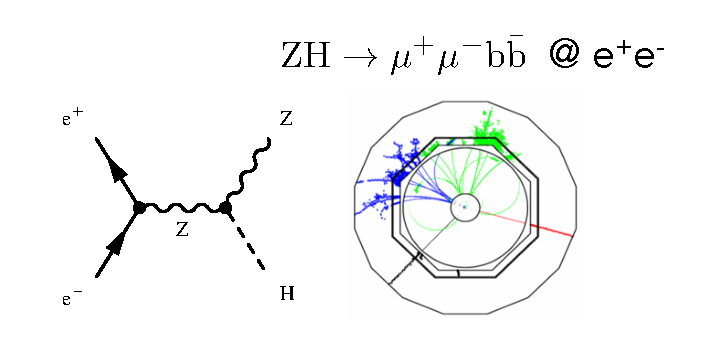
\includegraphics[width=0.6\textwidth]{figures/leptonColliders.pdf}

  \end{columns}


  \begin{columns}[t]
    \column{0.5\textwidth}

    \begin{itemize}
    \item Protons $\Rightarrow$ compound objects
      \begin{itemize}
      \item Unknown event-by-event initial states
      \item Limited achievable precision
      \end{itemize}
    \item High rates of QCD backgrounds
      \begin{itemize}
      \item Complex triggering schemes
      \item High levels of radiation
      \end{itemize}
    \item High cross-sections for coloured-states
    \item High-energy circular pp colliders are feasible
    \end{itemize}

    \column{0.5\textwidth}

    \begin{itemize}
    \item Electrons/positrons $\Rightarrow$ point like
      \begin{itemize}
      \item Well-defined initial states (energy, polarisation)
      \item High-precision measurements
      \end{itemize}
    \item Cleaner experimental environment
      \begin{itemize}
      \item Trigger-less readout
      \item Low levels of radiation
      \end{itemize}
    \item Superior sensitivity for electro-weak states
    \item High-energy $e^+e^-$ collisions ($\geq350\,\tev$) require
      linear colliders
    \end{itemize}

  \end{columns}

\end{frame}


%%%%%%%%%%%%%%%%%%%%%%%%%%%%%
%         SLIDE             %
%%%%%%%%%%%%%%%%%%%%%%%%%%%%%
\begin{frame}
  \frametitle{High-energy $e^+e^-$ colliders studies at CERN}

  \begin{columns}
    \column{0.6\textwidth}
    \begin{itemize}
    \item The Compact LInear Collider (CLIC)
      \begin{itemize}
      \item An $e^{+}e^{-}$ linear collider for the post HL-LHC period.
      \item Energy range $\sqrt{s}$ : \textcolor{blue}{$380\,\gev$} to
        \textcolor{blue}{$3\,\tev$}
        \begin{itemize} 
        \item Two-beam acceleration scheme with gradients of $\sim$100~MV/m.
        \end{itemize}
      \item Precision measurements of:
        \begin{itemize}
        \item Standard Model processes (Higgs, top).
        \item New physics potentially discovered at 13~TeV LHC.
        \item Search for new physics: unique sensitivity to particles with
          electroweak charge.
        \end{itemize}
      \end{itemize}
    \end{itemize}

    \column{0.4\textwidth}
    \begin{tikzpicture}
      \node[anchor=south west,inner sep=0] (image) at (0,
      0){\includegraphics[width=\textwidth]{../figures/CLIC/staging.pdf}};
      \begin{scope}[x={(image.south east)},y={(image.north west)}]
        \node[above, color=white] at (0.5, 0.001) {\textbf{48 km tunnel at 3 TeV stage}};
      \end{scope}
    \end{tikzpicture}
  \end{columns}
  
  \begin{columns}
    \column{0.7\textwidth}

    \begin{itemize}
    \item The Future Circular Collider (FCC-ee):
      \begin{itemize}
      \item Lepton collider in a new 80-100~km tunnel around CERN.
      \item Energy range $\sqrt{s}$: from $90\,\gev$ to $350\,\gev$.
      \item FCC-hh: for proton-proton collisions $\sqrt{s}$ is up to $100\,\tev$.
      \end{itemize}
    \end{itemize}

    \column{0.3\textwidth}
    \centering
    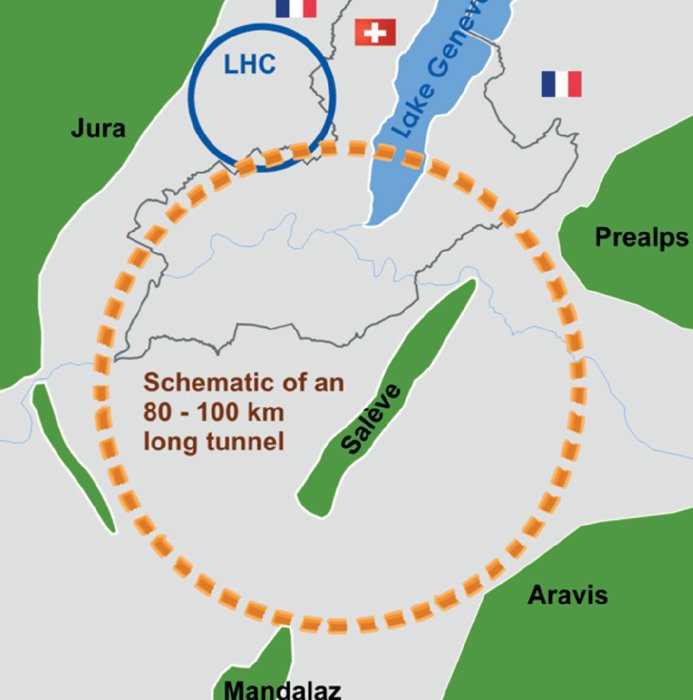
\includegraphics[width=0.9\textwidth]{figures/FCC}

  \end{columns}

\end{frame}

%%%%%%%%%%%%%%%%%%%%%%%%%%%%%
%         SLIDE             %
%%%%%%%%%%%%%%%%%%%%%%%%%%%%%
\subsection{CLIC beam profile}
\begin{frame}
  \frametitle{Beam profile for CLIC}

 \begin{columns}
    \column{0.5\textwidth}
    \begin{tikzpicture}
      \node[anchor=south west,inner sep=0] (image) at (0,
      0){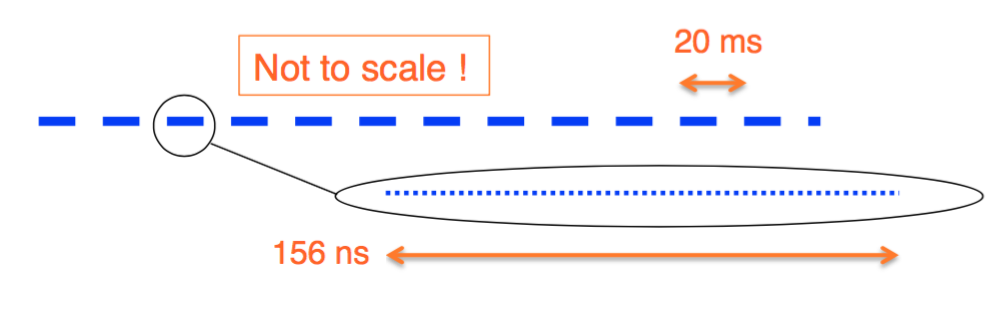
\includegraphics[width=\textwidth]{figures/CLICbeam.png}};
      \begin{scope}[x={(image.south east)},y={(image.north west)}]
        \node[above, color=blue] at (0.5, 0.9) {\textbf{CLIC bunch
            structure}};
        % \node[above, color=Orange] at (0.65, 0.05) {\tiny{1 train=312 bunches
        %     with 0.5~ns spacing}};
      \end{scope}
    \end{tikzpicture}

    \begin{itemize}
    \item 1 train consists of \textcolor{blue}{312} bunches with \textcolor{blue}{0.5}~ns spacing.
    \end{itemize}

    \centering
    \resizebox{0.9\columnwidth}{!}{\begin{tabular}{l c c} 
                                     \toprule 
                                     & CLIC at $\sqrt{s}=3\,\tev$ & LHC at $\sqrt{s}=13\,\tev$\\
                                     \midrule
                                     Colliding particles & electron-positron & proton-proton \\
                                     Instantaneous luminosity $\mathcal{L}$ & $6\times10^{34}$ \inversecmsquaredsec & $1\times10^{34}$ \inversecmsquaredsec \\
                                     Bunch-crossing separation & 0.5~ns & 25~ns \\
                                     Bunches per train & 312 & Not applicable \\
                                     Train duration & 156~ns & Not applicable \\
                                     Train repetition & 50~Hz & Not applicable \\
                                     IP size in x / y / z directions & 45~nm / 1~nm / $44\,\micron$ & $15\,\micron$ / $15\,\micron$ / 50~cm \\
                                     \bottomrule
                                   \end{tabular}}

    \column{0.5\textwidth}
    \centering
    \begin{itemize}
    \item \textcolor{Red}{Bunch separation and train duration: drive timing resolution requirements for the detectors.}
    \item \textcolor{Green}{Very small beam sizes at the interaction
        point} $\Rightarrow$ beam-induced backgrounds:
      \begin{itemize}
      \item \textcolor{blue}{$e^{+}e^{-}$ pairs}: low \pT, forward peaked, limits the inner radius of the VXD.
      \item \textcolor{blue}{$\gamma\gamma\rightarrow$hadrons}: larger \pT particles.
      \end{itemize}      
    \end{itemize}

  \end{columns}

  \begin{itemize}
  \item Short train duration implies:
    \begin{itemize}
    \item triggerless readout of the detectors.
    \item power pulsing: allows to reduce the average power dissipation.
    \end{itemize}
  \end{itemize}

\end{frame}


%%%%%%%%%%%%%%%%%%%%%%%%%%%%%
%         SLIDE             %
%%%%%%%%%%%%%%%%%%%%%%%%%%%%%
\section{Requirements}
\begin{frame}
  \frametitle{The CLIC detector}

  \begin{columns}
    \column{0.5\textwidth}
    \begin{tikzpicture}
      \node[anchor=south west,inner sep=0] (image) at (0,
      0){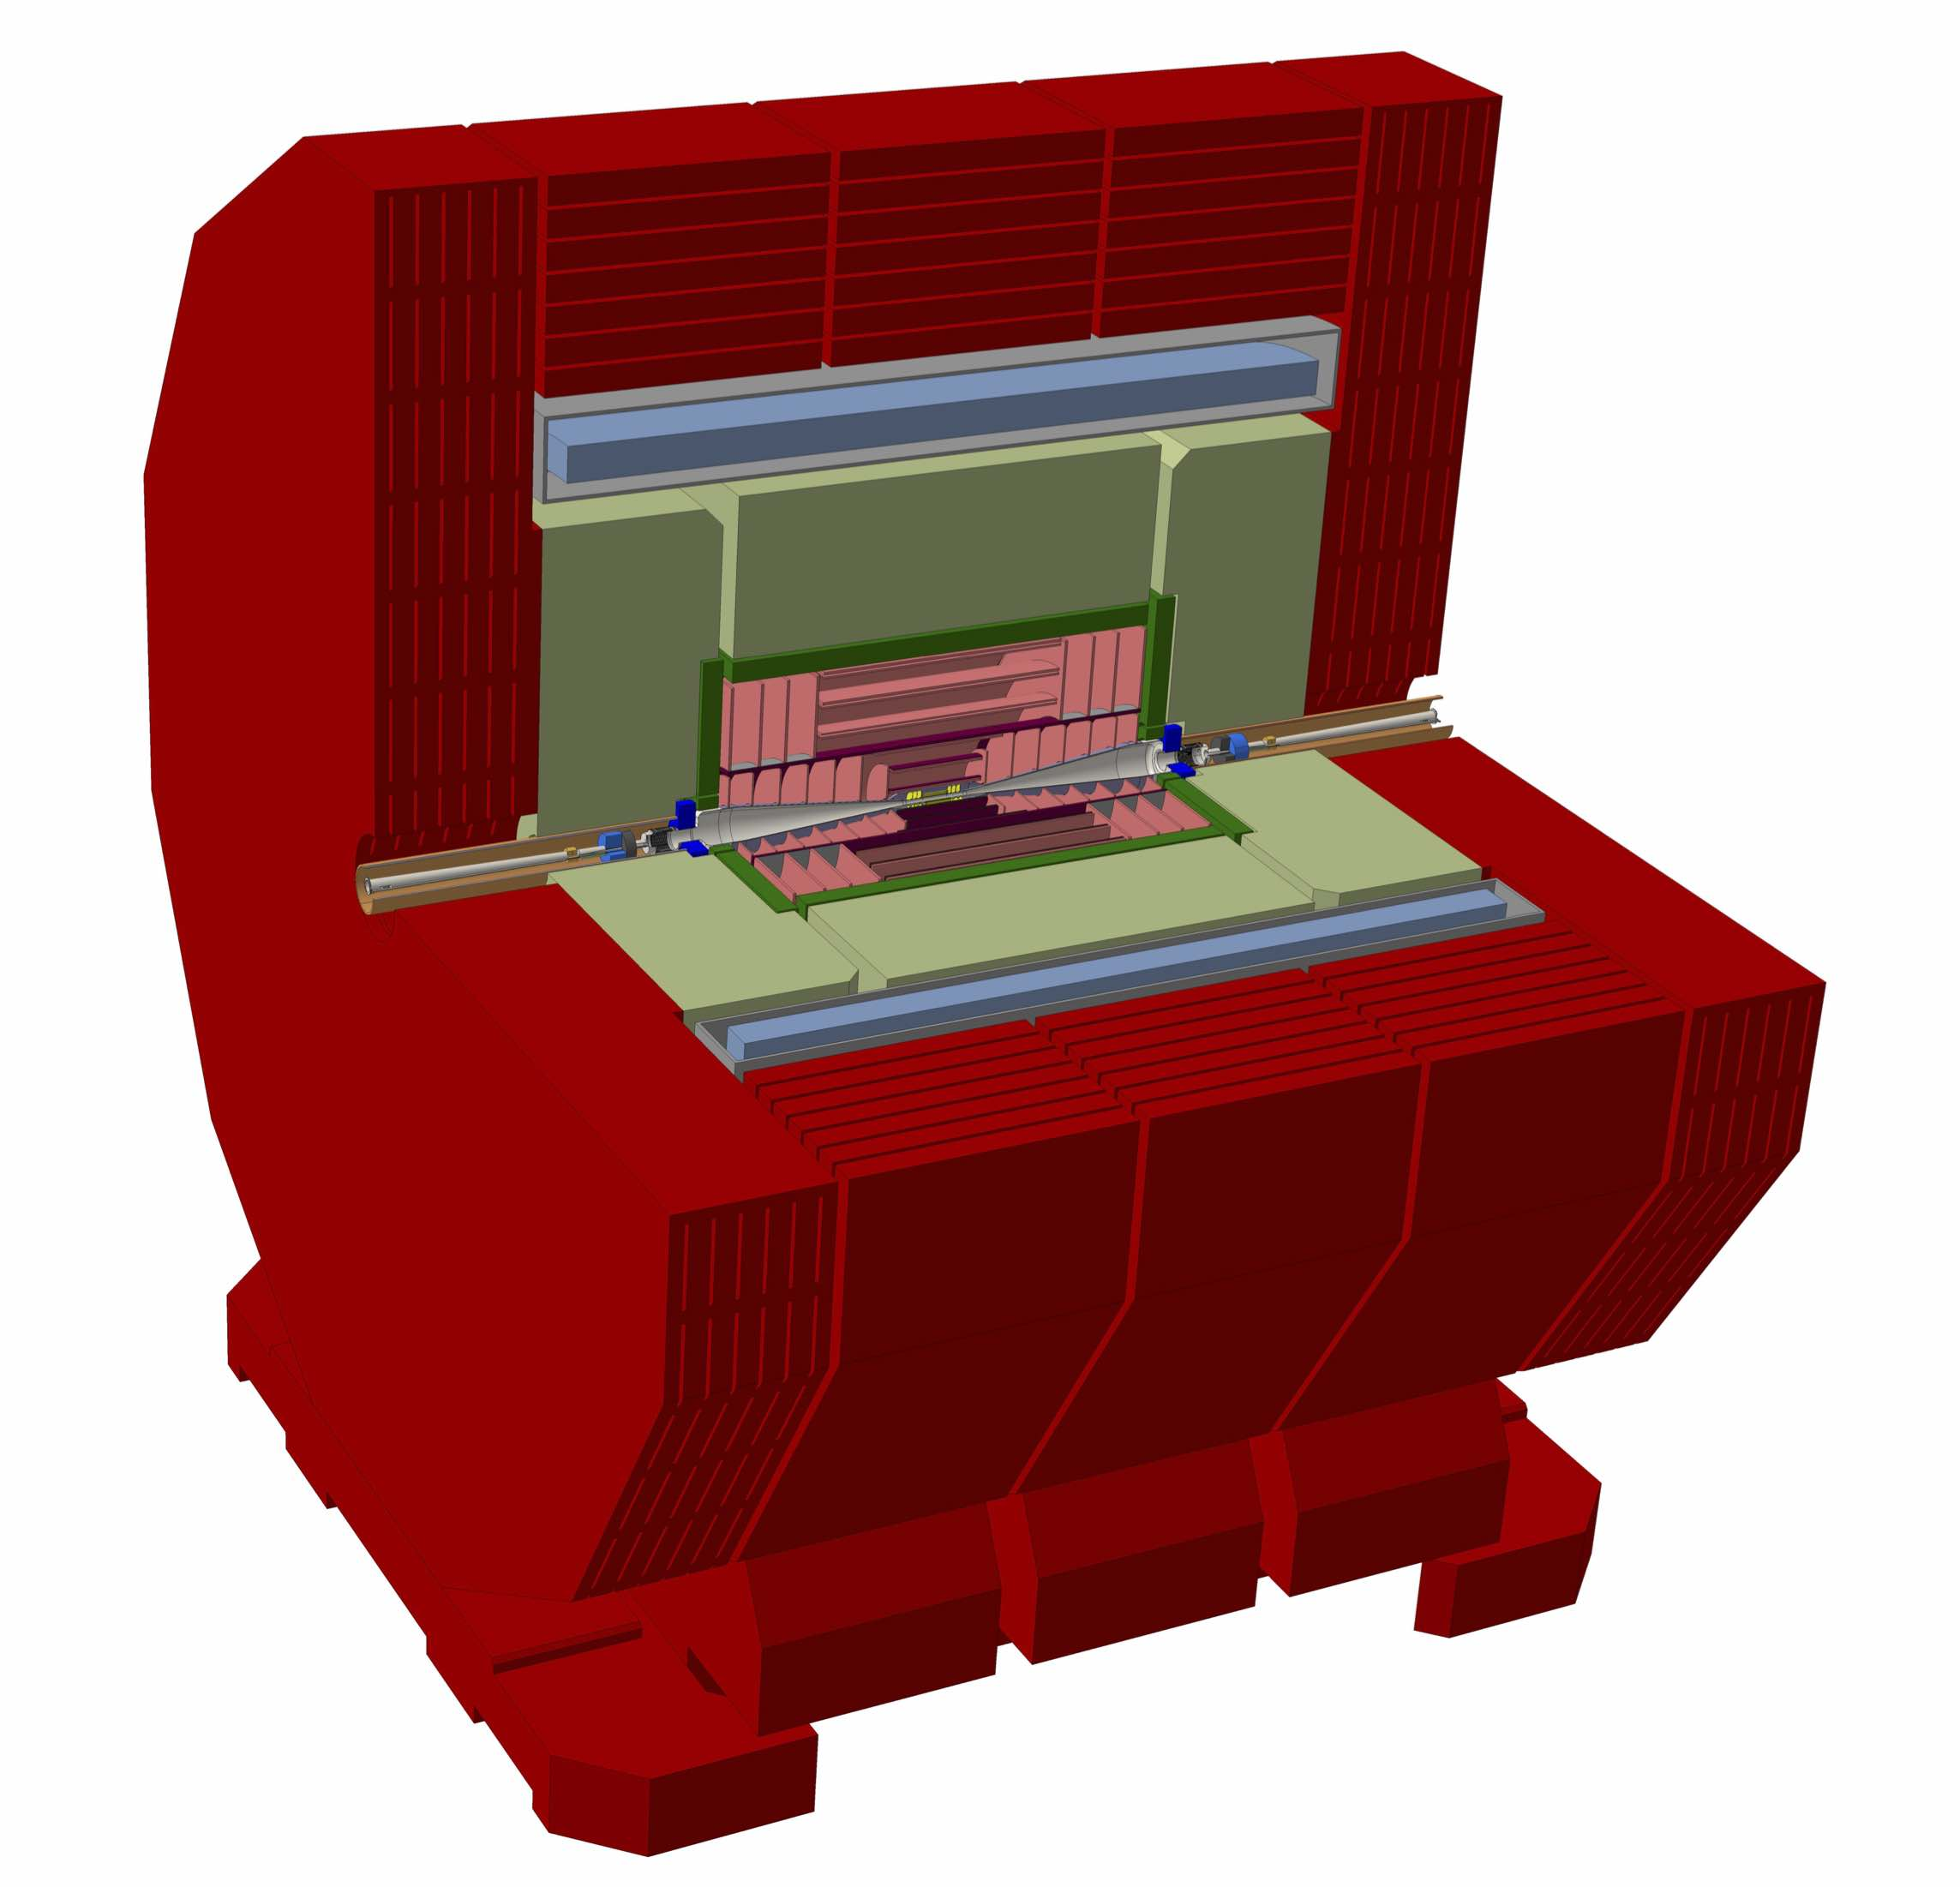
\includegraphics[width=\textwidth]{figures/CLIC_detector_2016.jpg}};
      \begin{scope}[x={(image.south east)},y={(image.north west)}]

        % \draw[help lines,xstep=.1,ystep=.1] (0, 0) grid (1,1);
        % \foreach \x in {0,1,...,9} { \node [anchor=north] at (\x/10,0) {0.\x}; }
        % \foreach \y in {0,1,...,9} { \node [anchor=east] at (0,\y/10)
        %   {0.\y}; }

        \draw[<->,line width=0.5pt] (0.32, 0.0) -- (0.8, 0.13);
        \node[color=black] at (0.6, 0.02) {11.4~m};

        \draw[<->,line width=0.5pt] (0.04, 0.17) -- (0.04, 0.9);
        \node[color=black, rotate=90] at (0.01, 0.5) {12.9~m};
      \end{scope}
    \end{tikzpicture}

    \column{0.5\textwidth}
    \begin{itemize}
    \item CMS-like detector (????? TO BE CHECKED)
    \item Silicon-based and low mass tracking system.
    \item Fine-grained calorimetry system (ECAL and HCAL) optimised
      for particle flow analysis (PFA).
    \item Superconducting solenoid magnet: B=4~T.
    \item Return iron yoke with detectors for muon identification.
    \item Forward region with LumiCal (luminosity monitoring) and
      BeamCal (beam calorimeter).
    \end{itemize}

  \end{columns}

\end{frame}

%%%%%%%%%%%%%%%%%%%%%%%%%%%%%
%         SLIDE             %
%%%%%%%%%%%%%%%%%%%%%%%%%%%%%
\begin{frame}
  \frametitle{Requirements for the vertex detector}
\end{frame}


%-------------------------------------------------------
%-------------------------------------------------------
\section{R\&D on sensor and readout technologies}
%-------------------------------------------------------
\subsection{Thin planar sensors}
\begin{frame}
  \frametitle{Thin planar sensors}
\end{frame}
%-------------------------------------------------------
\subsection{The Timepix3 hybrid readout ASIC}
\begin{frame}
  \frametitle{The Timepix3 hybrid readout ASICs}
\end{frame}
%-------------------------------------------------------
\begin{frame}
  \frametitle{Assembly calibration}
\end{frame}

%-------------------------------------------------------
%-------------------------------------------------------
\section{Simulation}
\begin{frame}
  \frametitle{Simulation and reconstruction}
\end{frame}


%-------------------------------------------------------
%-------------------------------------------------------
\section{Timepix3 beam telescope}
\begin{frame}
  \frametitle{Timepix3 beam telescope}
\end{frame}

%-------------------------------------------------------
%-------------------------------------------------------
\section{Thin sensors studies}
\begin{frame}
  \frametitle{Thin sensors studies}
\end{frame}

%-------------------------------------------------------
%-------------------------------------------------------
\section{Active edge sensors}
\begin{frame}
  \frametitle{Active edge sensors}
\end{frame}

%-------------------------------------------------------
%-------------------------------------------------------
\label{lastslide}
\section{Conclusions}
\begin{frame}
  \frametitle{Conclusions}
\end{frame}